\section{Introduction}

  The Muon g-2 Experiment at Fermilab will use tracking detectors in order to measure positron trajectories for the purpose of determining the beam distribution and its characteristics, both for the final $\omega_{a}$ result and for general beam diagnostics. A fraction of positrons originating from decaying muons will pass through the trackers. By fitting these tracks and extrapolating back to the average decay point, the beam can be characerized in a non-destructive fashion. The tracking can be done independently from the calorimeters in order to cross-check, or combined with them in order to provide the muon distribution that the calorimeters see for the direct $\omega_{a}$ calculation. It is arguable that this is the most important duty of the trackers. (Note that the integration of the two detector systems in the code has not been initiated.) It is also worth noting that there is a large percentage of tracks that hit the calorimeters hit zero or a small number of tracking modules, which this fitting code is not capable of handling.

  Each tracker module consists of 4 layers of 32 straws with a stereo angle of 7.5 degrees, the first two ``U'' layers oriented with the tops of the straws at a greater radial position, and the second two ``V'' layers oriented with the bottoms of the straws at a greater radial position. A tracking module is shown in Figure \ref{fig:tracker}. There are 3 tracker stations located at the 0, 12th, and 18th sections of the ring, counting clockwise from the top most point of the ring where the inflector resides. (Station 18 has been installed at time of writing, with station 0 planned for the fall. Station 12 is slated for the future sometime.) Each station consists of 8 tracking modules arranged in a staircase pattern that follows the curvature of the ring as seen in Figure \ref{fig:staircase}. Further hardware and electronics information regarding the trackers will be omitted in this document.

\begin{figure}[]
\caption{Shown is a picture of one of the many tracking modules used in the Muon g-2 experiment. The first layer of straws with a stereo angle of 7.5 degrees can be seen, with the other 3 straw layers hiding behind it. The beam direction is roughly into the page in this picture, and this view is what the decay positrons will see. Picture provided by James.}
\centering
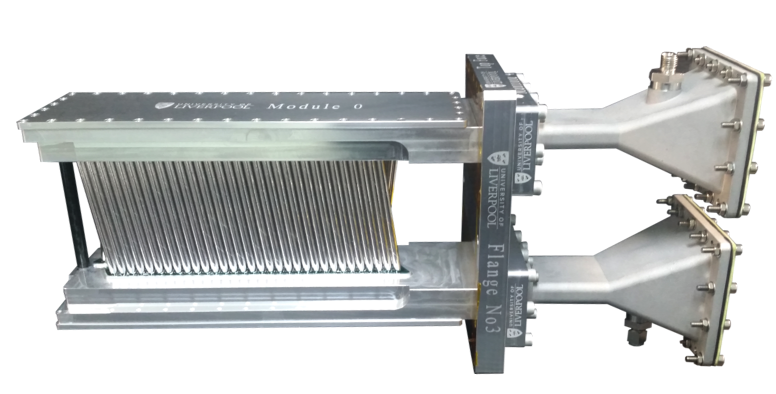
\includegraphics[width=0.9\textwidth]{Tracker}
\label{fig:tracker}
\end{figure}

\begin{figure}[]
\caption{Tracker modules are arranged in the shown staircase pattern. In green and dark blue is the edge of the vacuum chamber (where the dark blue identifies the modification that was made to the old vacuum chambers), and it can be seen that vacuum chamber walls lie at the ends of the outside tracking modules. The position of a calorimeter can be seen in teal at the right. The dark red spots are the locations of the pole tips.}
\centering
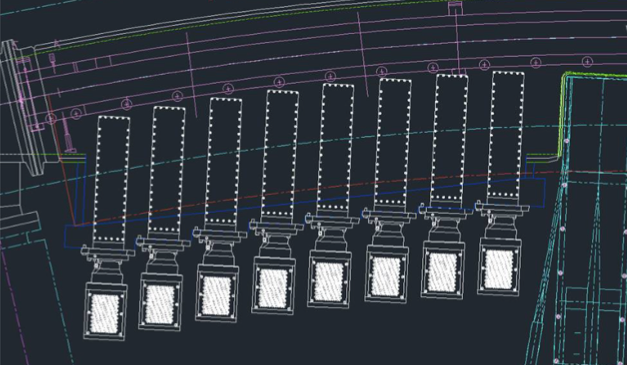
\includegraphics[width=0.9\textwidth]{trackerStation}
\label{fig:staircase}
\end{figure}


  Because of the proximity of the trackers to the muon beam, they will lie within a region of varying field. The radial field of the trackers rises from 0 Tesla at the outer ends to roughly .3 Tesla at the inner top and bottom ends, and the vertical field drops approximately 50\% from the storage dipole field of 1.451 Tesla. Shown in Figures \ref{fig:operaBy} and \ref{fig:operaBx} is the location of the tracker with respect to the horizontal and vertical fields respectively. If one thing can be said to be special to g-2 when it comes to tracking it is these large field gradients over the tracking detector region and several meter long extrapolation distance back to the muon decay point. This is one of the main motivations for using the Geane (Geometry and Error Propagation) fitting algorithm and routines, which has direct access to the field. 


\begin{figure}[]
\caption{Shown is the vertical field of the g-2 magnet in and around the storage region as calculated in Opera 2D. The center of the storage region lies at 7.112 m along the x axis. The black box shows the rough location of the tracker with respect to the field (size exaggerated slightly). It can be seen that there is a large inhomogeneity within the tracker space, goring from left to right.}
\centering
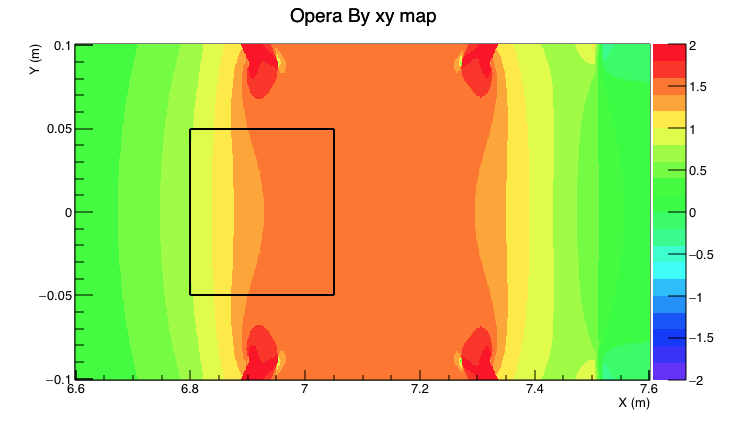
\includegraphics[width=0.9\textwidth]{operaBy}
\label{fig:operaBy}
\end{figure}

\begin{figure}[]
\caption{Shown is the radial field of the g-2 magnet in and around the storage region as calculated in Opera 2D. The center of the storage region lies at 7.112 m along the x axis. The black box shows the rough location of the tracker with respect to the field (size exaggerated slightly). It can be seen that there is a large homogeneity at the inner upper and lower ends compared to the right center. The shape of the pole pieces and tips can readily be seen.}
\centering
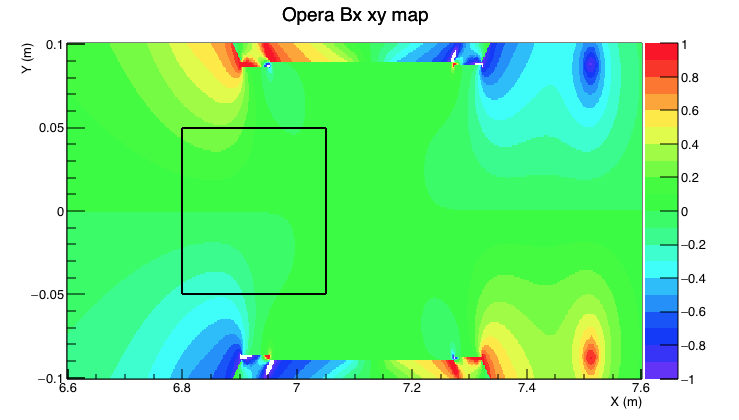
\includegraphics[width=0.9\textwidth]{operaBx}
\label{fig:operaBx}
\end{figure}

  The Geane fitting routines originated in Fortran with the EMC collaboration, and was used in the precursor E821 experiment as well as the PANDA experiment with some success. (cite stuff here?) (There might be some other instances of its use as well.) The core error propagation routines were at some point added to Geant4 under the error\_propagation directory which is included in all default installs. The tracking code strengths lie with its direct implementation and access to the Geant4 geometry and field, and its ability to handle the field inhomogeneties. The Geane algorithm code which makes use of the Geant4 error\_propagation routines follows the structure of \cite{geanemanual} and is detailed in the \hyperref[sec:Formalism]{Formalism} section in this paper. It is a relatively straight forward least squares global $\chi^{2}$ minimization algorithm. 

